%%
%% This is file `sample-sigconf.tex',
%% generated with the docstrip utility.
%%
%% The original source files were:
%%
%% samples.dtx  (with options: `sigconf')
%% 
%% IMPORTANT NOTICE:
%% 
%% For the copyright see the source file.
%% 
%% Any modified versions of this file must be renamed
%% with new filenames distinct from sample-sigconf.tex.
%% 
%% For distribution of the original source see the terms
%% for copying and modification in the file samples.dtx.
%% 
%% This generated file may be distributed as long as the
%% original source files, as listed above, are part of the
%% same distribution. (The sources need not necessarily be
%% in the same archive or directory.)
%%
%%
%% Commands for TeXCount
%TC:macro \cite [option:text,text]
%TC:macro \citep [option:text,text]
%TC:macro \citet [option:text,text]
%TC:envir table 0 1
%TC:envir table* 0 1
%TC:envir tabular [ignore] word
%TC:envir displaymath 0 word
%TC:envir math 0 word
%TC:envir comment 0 0
%%
%%
%% The first command in your LaTeX source must be the \documentclass
%% command.
%%
%% For submission and review of your manuscript please change the
%% command to \documentclass[manuscript, screen, review]{acmart}.
%%
%% When submitting camera ready or to TAPS, please change the command
%% to \documentclass[sigconf]{acmart} or whichever template is required
%% for your publication.
%%
%%
\documentclass[sigconf]{acmart}

\usepackage{bm}
\usepackage{algorithm}
\usepackage[noEnd=True]{algpseudocodex}
\usepackage{tikz}
\usepackage{listings}
\usepackage{float}
\usepackage{caption}
\usepackage{subcaption}
\usepackage{graphicx}
\usepackage{xcolor}
\usepackage{multirow,siunitx}
\floatstyle{plain}
\newfloat{Figure}{t}{myc}

\definecolor{dkgreen}{rgb}{0,0.6,0}
\definecolor{gray}{rgb}{0.5,0.5,0.5}
\definecolor{mauve}{rgb}{0.58,0,0.82}
\definecolor{verylightgray}{rgb}{.97,.97,.97}

\lstset{frame=tb,
  language=Python,
  aboveskip=3mm,
  belowskip=3mm,
  showstringspaces=false,
  columns=flexible,
  basicstyle={\small\ttfamily},
  numbers=none,
  backgroundcolor = \color{verylightgray},
  numberstyle=\tiny\color{gray},
  keywordstyle=\color{blue},
  commentstyle=\color{black},
  stringstyle=\color{black},
  breaklines=true,
  breakautoindent=false,
  breakindent=0pt,
  breakatwhitespace=true,
  tabsize=3
}

\usepackage{pgfplots}
\pgfplotsset{
    width=8cm,
    compat=1.9,
    legend style={
      fill,
      at={(0.50,-0.35)},
      legend columns=1,
      legend cell align=left,
      anchor=north
      }
    }
%%
%% \BibTeX command to typeset BibTeX logo in the docs
\AtBeginDocument{%
  \providecommand\BibTeX{{%
    Bib\TeX}}}

%% Rights management information.  This information is sent to you
%% when you complete the rights form.  These commands have SAMPLE
%% values in them; it is your responsibility as an author to replace
%% the commands and values with those provided to you when you
%% complete the rights form.
\setcopyright{acmlicensed}
\copyrightyear{2018}
\acmYear{2018}
\acmDOI{XXXXXXX.XXXXXXX}

%% These commands are for a PROCEEDINGS abstract or paper.
\acmConference[Conference acronym 'XX]{Make sure to enter the correct
  conference title from your rights confirmation emai}{June 03--05,
  2018}{Woodstock, NY}
%%
%%  Uncomment \acmBooktitle if the title of the proceedings is different
%%  from ``Proceedings of ...''!
%%
%%\acmBooktitle{Woodstock '18: ACM Symposium on Neural Gaze Detection,
%%  June 03--05, 2018, Woodstock, NY}
\acmISBN{978-1-4503-XXXX-X/18/06}


%%
%% Submission ID.
%% Use this when submitting an article to a sponsored event. You'll
%% receive a unique submission ID from the organizers
%% of the event, and this ID should be used as the parameter to this command.
%%\acmSubmissionID{123-A56-BU3}

%%
%% For managing citations, it is recommended to use bibliography
%% files in BibTeX format.
%%
%% You can then either use BibTeX with the ACM-Reference-Format style,
%% or BibLaTeX with the acmnumeric or acmauthoryear sytles, that include
%% support for advanced citation of software artefact from the
%% biblatex-software package, also separately available on CTAN.
%%
%% Look at the sample-*-biblatex.tex files for templates showcasing
%% the biblatex styles.
%%

%%
%% The majority of ACM publications use numbered citations and
%% references.  The command \citestyle{authoryear} switches to the
%% "author year" style.
%%
%% If you are preparing content for an event
%% sponsored by ACM SIGGRAPH, you must use the "author year" style of
%% citations and references.
%% Uncommenting
%% the next command will enable that style.
%%\citestyle{acmauthoryear}


%%
%% end of the preamble, start of the body of the document source.
\begin{document}

%%
%% The "title" command has an optional parameter,
%% allowing the author to define a "short title" to be used in page headers.
\title{CiteQ: Analysis on Citation Sentiment: University of Waterloo Computer Science Faculty Case Study} 

%%
%% The "author" command and its associated commands are used to define
%% the authors and their affiliations.
%% Of note is the shared affiliation of the first two authors, and the
%% "authornote" and "authornotemark" commands
%% used to denote shared contribution to the research.
\author{Onur Eren Arpaci}
\email{oearpaci@uwaterloo.ca}
\affiliation{%
  \institution{University of Waterloo}
  \streetaddress{200 University Ave W}
  \city{Waterloo}
  \state{Ontario}
  \country{Canada}
  \postcode{N2L 3G1}
}

%%
%% By default, the full list of authors will be used in the page
%% headers. Often, this list is too long, and will overlap
%% other information printed in the page headers. This command allows
%% the author to define a more concise list
%% of authors' names for this purpose.
\renewcommand{\shortauthors}{Arpaci}

%%
%% The abstract is a short summary of the work to be presented in the
%% article.
\begin{abstract}
While citation count and H-index is the most important metrics for measuring impact in Science, the intention of the given citation is usually overlooked. To examine the affects of citation sentiments on academic success, this paper conducts a large scale empirical study on University of Waterloo Computer Science faculty members' publication data. We show a negative correlation between H-index and the percentage of negative citations given by that researcher. We also show a positive correlation between number of papers published by a researcher and percentage of neutral citations given by that researcher. In addition we discuss the changes in the distribution of citation sentiments over time and the differences between same institution and different institution citation sentiments. We also provide a dataset of 9,438 papers' metadata and 697,609 citations with their citation sentiments for future research.
\end{abstract}

%%
%% The code below is generated by the tool at http://dl.acm.org/ccs.cfm.
%% Please copy and paste the code instead of the example below.
%%
\begin{CCSXML}
    <ccs2012>
       <concept>
           <concept_id>10002951.10003317</concept_id>
           <concept_desc>Information systems~Information retrieval</concept_desc>
           <concept_significance>300</concept_significance>
           </concept>
       <concept>
           <concept_id>10002944.10011123.10011131</concept_id>
           <concept_desc>General and reference~Experimentation</concept_desc>
           <concept_significance>500</concept_significance>
           </concept>
       <concept>
           <concept_id>10003456.10010927.10003619</concept_id>
           <concept_desc>Social and professional topics~Cultural characteristics</concept_desc>
           <concept_significance>100</concept_significance>
           </concept>
     </ccs2012>
\end{CCSXML}
    
\ccsdesc[300]{Information systems~Information retrieval}
\ccsdesc[500]{General and reference~Experimentation}
\ccsdesc[100]{Social and professional topics~Cultural characteristics}

%%
%% Keywords. The author(s) should pick words that accurately describe
%% the work being presented. Separate the keywords with commas.
\keywords{Citation Sentiment, Citation Analysis, Citation Trends, LLM classification}
%% A "teaser" image appears between the author and affiliation
%% information and the body of the document, and typically spans the
%% page.

\received{20 February 2007}
\received[revised]{12 March 2009}
\received[accepted]{5 June 2009}

%%
%% This command processes the author and affiliation and title
%% information and builds the first part of the formatted document.
\maketitle

\section{Introduction}
The predominant and widely recognized scientometric indicator is the number 
of citations a paper garners. Nevertheless, it's crucial to acknowledge that 
papers can be cited for diverse reasons. A citation may stem from a paper 
serving as the foundational work for current research, acting as a competitor 
in the field, or being subject to critique. 

The purpose of this paper is to study the citation sentiments and its affects
on citation counts. We aim to answer the following research 
questions:

\begin{enumerate}
    \item[RQ1] Do the citation sentiments affect the total number of
    citations a paper or a researcher receives? (i.e. is there a karma effect?)
    \item[RQ2] How does the distribution of citation sentiments change over the
    duration of a researcher's career?
    \item[RQ3] How did the distribution of citation sentiments change over time?
    \item[RQ4] Is there any difference in the distribution of citation sentiments
    between same institution researchers and different institution researchers? 
\end{enumerate} 

We collected the publication and citation data of
the University of Waterloo Computer Science faculty members. We then used
the large language model (LLM) Solar 10.7B \cite{upstage2023solar} to classify the citation 
sentiments of each paper. We then analyzed this data to answer the research questions.

\section{Related Work}
There is a large body of research on citation analysis. Most of these studies use the ACL Anthology \cite{bird2008acl} as their dataset. ACL Anthology is a dataset of NLP papers and their citations. Using the ACL Anthology creates two main differences from our study. First, it provides more contextual metadata about the citations than our dataset, such as the position of the citation in the paper, the section of the paper that the citation is in, etc. Second, it provides a large enough training dataset to train or finetune any kind of model, which our dataset also lacks. \cite{athar2011sentiment, athar2012context, abu2013purpose, hernandez2015citation} are some of the studies that use the ACL Anthology dataset. They are generally focusing on the task of citation sentiment classification itself and they do not analyze the output of this classification. None of the studies we have found use LLMs for classification. Most use sentence or word embeddings.

\cite{yan2020relationship}, \cite{yan2020authors} are some of the studies that analyze the citation sentiment classification output. \cite{yan2020relationship} analyze the relationship between journal impact and the citation sentiment. They use PubMed Central dataset \cite{pubmed} for this study. \cite{yan2020authors} analyze the relationship between Nobel prize winners and their citation sentiments pre and post Nobel prize. They manually gather a 100 paper dataset for this study.


\begin{figure}[h]
  \centering
  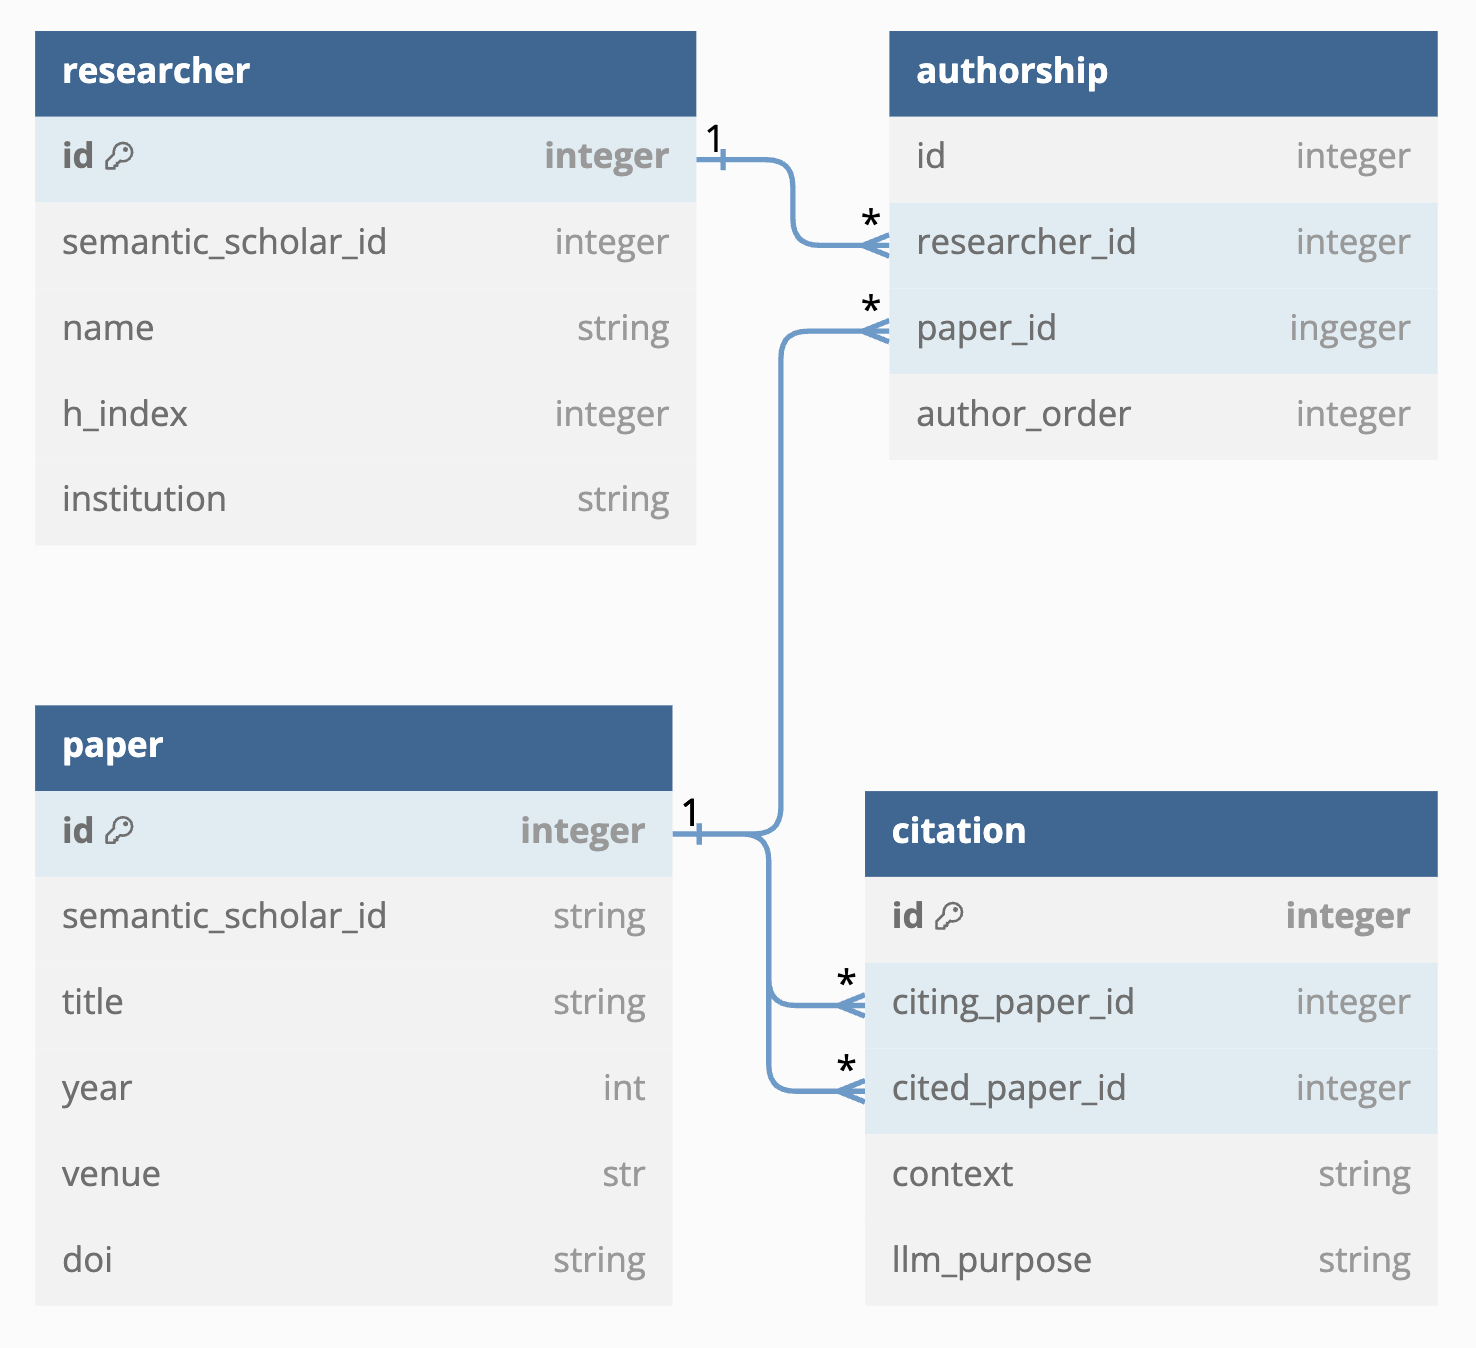
\includegraphics[width=\linewidth]{citeq-scheme.png}
  \caption{CiteQ database scheme}
  \label{fig:citeq-scheme}
\end{figure}

\sisetup{table-format=2.2} 
\begin{table*}
\centering
    \begin{tabular}{|l|S|S|S|S|S|S|S|S|S|S|}           \hline 
\multirow{2}{*}{type}    & \multicolumn{2}{c|}{Positive}    &\multicolumn{2}{c|}{Negative}  &\multicolumn{2}{c|}{Neutral}  &\multicolumn{2}{c|}{Bad Context} &\multicolumn{2}{c|}{\textbf{Average}}  \\   \cline{2-11}
  &{Prec.} & {Rec.} & {Prec.}  & {Rec.} &{Prec.}  & {Rec.} &{Prec.} &{Rec.}  &{Prec.}  & {Rec.}         \\   \hline 
Solar 10.7B& 0.68 &0.41 & 0.67 & \textbf{0.67} & \textbf{0.47} & 0.87 & 0.90 & 0.44 &0.68 & \textbf{0.60} \\ \hline  
GPT-4.5 & \textbf{0.87} & 0.19 & 0.71 & 0.62 & 0.43 & \textbf{0.96} & 0.92 & \textbf{0.52} & \textbf{0.73} & 0.57 \\ \hline
GPT-3.5 & 0.50 & \textbf{0.95} & \textbf{0.80} & 0.50 & 0.36 & 0.21 & \textbf{1.00} & 0.26 & 0.66 & 0.47\\   \hline
mistral 7x8B & 0.70 & 0.38 & 0.71 & 0.56 & 0.41 & 0.84 & 0.60 & 0.26 & 0.60 & 0.51\\ \hline
llama2 7B & 0.39 & 0.75 & 0.60 & 0.375 & 0.34 & 0.25 & \textbf{1.00} & 0.04 & 0.58 & 0.35\\   \hline 
mistral & 0.48 & 0.27 & 0.36 & 0.50 & 0.43 & 0.87 & 0.75 & 0.13 & 0.50 & 0.44\\ \hline
 \end{tabular}
\caption{Evaluation results of the LLMs}
\label{table:evaluation}
\end{table*}

\section{Methodology}
\subsection{Data Collection}
We used the Semantic Scholar (SS) API to collect the publication and citation data of all current (as of this writing) members of the University of Waterloo Computer Science faculty members. SS provides an API endpoint to retrieve the context of a citation. We used this endpoint to retrieve the citation context of each citation
made by a faculty member or to a faculty member. In total we collected data about 96 faculty members, 9,438 papers, and 697,609 citations. We formed an SQLite database, with the scheme shown in Figure \ref{fig:citeq-scheme}, to facilitate flexible querying of the data. This database is publicly available at \url{https://github.com/onurerenarpaci/citeQ.git}.

\subsection{Citation Sentiment Classification}
We experimented with a number of LLMs including chatGPT-3.5 \cite{brown2020language}, chatGPT-4.5 \cite{openai2023gpt4}, mistral and mistral 7x8B \cite{jiang2023mistral}, llama2 \cite{touvron2023llama} and Solar 10.7B \cite{upstage2023solar}. Among these, only promising results were obtained from Solar 10.7B and \cite{openai2023gpt4}. Since with the size of the dataset we had, we could not afford to run the classification on GPT-4.5, so we chose Solar 10.7B as our LLM.

We used the following citation purpose classes: positive, neutral, negative, bad context. The positive class includes citations that are talking about the strengths of the paper, important it is. The negative class includes citations that are talking about the weaknesses of the paper, or talks about their solution being better than the paper's solution. The neutral class includes citations that are talking about the paper without any positive or negative sentiment. The bad context class is for badly captured citation contexts that do not contain any information about the citation sentiment. With the satisfactory precision on the bad context class, we removed all the citations labeled as bad context from our dataset for all the analysis we have conducted. You can see the prompt template we used in Appendix \ref{appendix:classification-prompt}.

We used 6 Nvidia A100 80GB GPUs to run the classification. The total inference time was 1 day and 4 hours.

\subsubsection{Evaluation}
We hand labeled 100 citations to evaluate the accuracy of the classification.
The results are shown in Table \ref{table:evaluation}. We can see that the Solar 10.7B has the highest average recall, and second highest average precision. We can also see that the Solar 10.7B has the most consistent scores among classes, which is important for our analysis. Therefore, we chose Solar 10.7B as our LLM.

\section{Results}

\begin{Figure}
  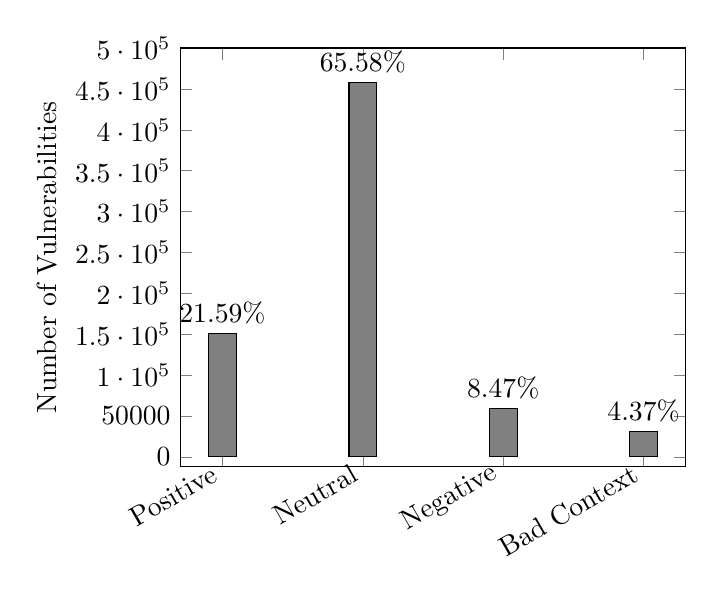
\begin{tikzpicture}
  \begin{axis}[
      symbolic x 
      coords={Positive, Neutral, Negative, Bad Context},
      scaled ticks=false,
      style={/pgf/number format/1000 sep=},
      xtick=data,
      xticklabel style = {rotate=30,anchor=east},
      ytick distance=50000,
      ylabel=Number of Vulnerabilities,
      point meta={(y/697609)*100},
      nodes near coords={\pgfmathprintnumber\pgfplotspointmeta\%}]
      \addplot[ybar,fill=gray] coordinates {
          (Positive, 150639)
          (Neutral, 457463)
          (Negative, 59054)
          (Bad Context, 30453)
      };
  \end{axis}
  \end{tikzpicture}
  \caption{Distribution of citation purposes}
  \label{graph:distribution}
\end{Figure}

\begin{figure*}
  \centering
  \begin{subfigure}{0.3\textwidth}
    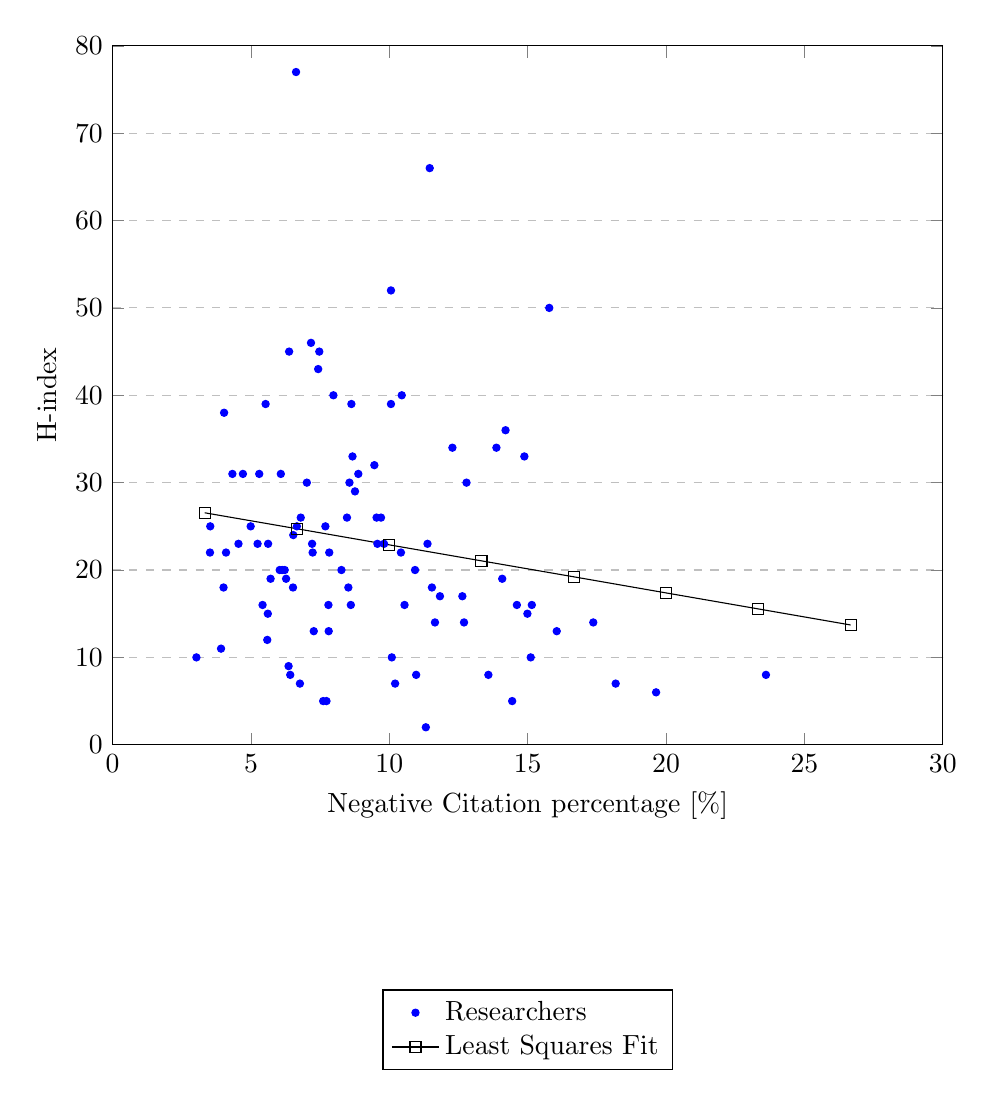
\begin{tikzpicture}
      \begin{axis}[
          width=(1\textwidth),
          xlabel={Negative Citation percentage [\%]},
          ylabel={H-index},
          xmin=0, xmax=30,
          ymin=0, ymax=80,
          xtick={0, 5, 10, 15, 20, 25, 30},
          ytick={0,10,20,30,40,50,60,70,80},
          ymajorgrids=true,
          grid style=dashed,
        ]
      
        \addplot[
          only marks, color=blue, mark size=1.3pt
          ]
          coordinates {
            (15.15,16)(10.55,16)(14.44,5)(7.21,23)(9.57,23)(7.83,22)(18.18,7)(8.52,18)(6.66,25)(3.92,11)(9.46,32)(6.8,26)(4.01,18)(11.46,66)(7.98,40)(7.73,5)(11.38,23)(12.7,14)(16.05,13)(6.53,24)(7.17,46)(5.53,39)(8.88,31)(10.06,39)(11.83,17)(5.42,16)(8.27,20)(5.59,12)(4.55,23)(10.45,40)(15.78,50)(14.08,19)(12.64,17)(7.23,22)(10.09,10)(6.36,9)(14.99,15)(14.88,33)(7.43,43)(6.77,7)(7.47,45)(8.47,26)(5.62,23)(4.71,31)(14.61,16)(14.2,36)(5.3,31)(9.81,23)(4.1,22)(7.8,16)(7.02,30)(8.63,39)(9.7,26)(11.65,14)(6.63,77)(13.58,8)(6.42,8)(3.52,22)(10.21,7)(7.27,13)(7.69,25)(17.37,14)(13.87,34)(12.28,34)(10.97,8)(5.24,23)(5.61,15)(6.22,20)(10.06,52)(6.38,45)(6.13,20)(11.54,18)(6.08,31)(6.52,18)(4.33,31)(4.03,38)(3.03,10)(7.61,5)(3.53,25)(10.42,22)(15.11,10)(8.56,30)(8.61,16)(8.67,33)(12.79,30)(7.81,13)(4.99,25)(6.04,20)(10.93,20)(11.32,2)(8.76,29)(23.61,8)(9.54,26)(19.64,6)(6.27,19)(5.71,19)
          };
          \addlegendentry{Researchers}
        
        \addplot[
          mark=square,
          ]
          coordinates {
            (3.33,26.55)(6.67,24.72)(10.0,22.88)(13.33,21.05)(16.67,19.22)(20.0,17.38)(23.33,15.55)(26.67,13.71)
          };
          \addlegendentry{Least Squares Fit}
          
      \end{axis}
    \end{tikzpicture}
    \caption{Negative citation percentage vs. H-index}
    \label{graph:negative-karma}
\end{subfigure}
\hfill
\begin{subfigure}{0.3\textwidth}
  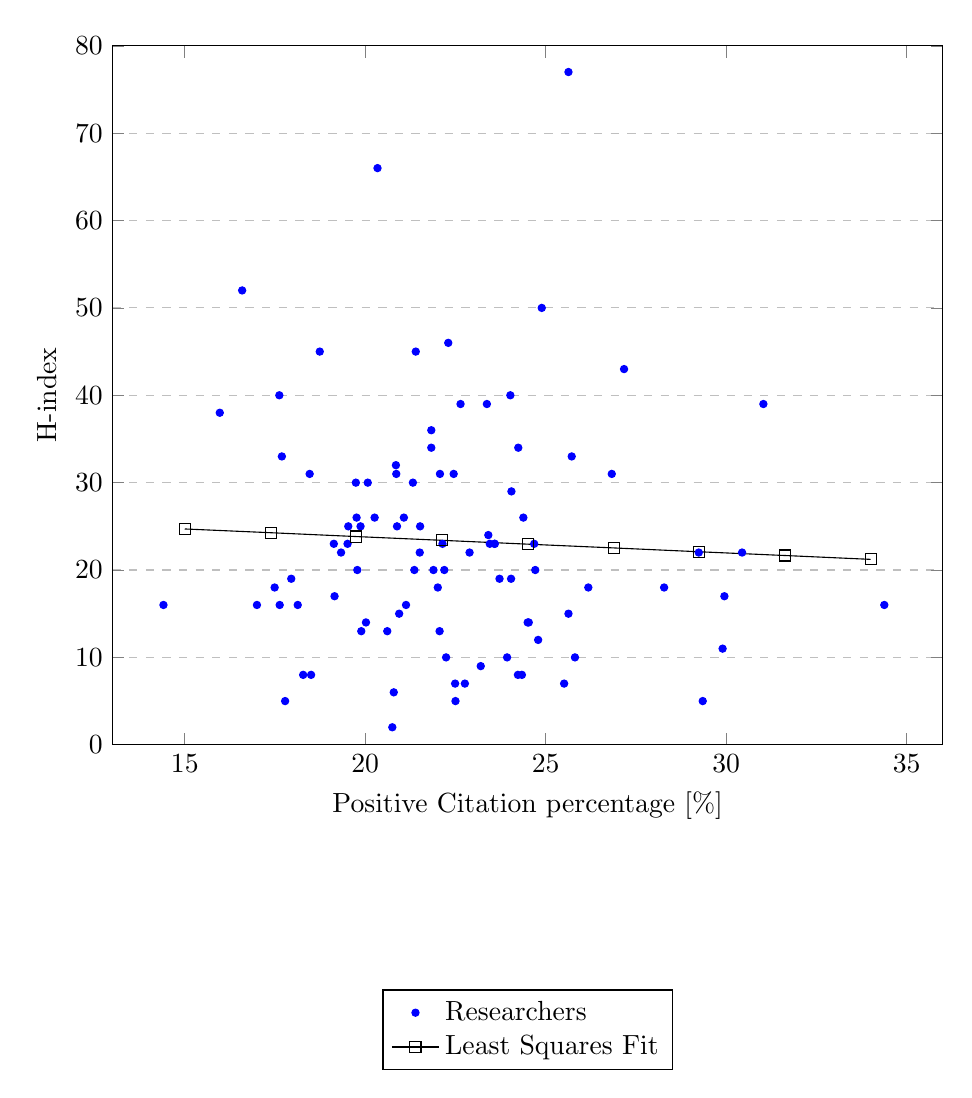
\begin{tikzpicture}
    \begin{axis}[
        width=(1\textwidth),
        xlabel={Positive Citation percentage [\%]},
        ylabel={H-index},
        xmin=13, xmax=36,
        ymin=0, ymax=80,
        xtick={10, 15, 20, 25, 30, 35},
        ytick={0,10,20,30,40,50,60,70,80},
        ymajorgrids=true,
        grid style=dashed,
    ]
    
    \addplot[
      only marks, color=blue, mark size=1.3pt
      ]
      coordinates {
        (14.41,16)(17.0,16)(17.78,5)(24.68,23)(19.13,23)(19.33,22)(22.76,7)(28.28,18)(19.87,25)(29.9,11)(20.85,32)(19.76,26)(26.18,18)(20.34,66)(24.02,40)(22.5,5)(22.14,23)(24.5,14)(19.89,13)(23.41,24)(22.3,46)(31.03,39)(26.83,31)(22.64,39)(19.15,17)(18.13,16)(21.89,20)(24.79,12)(23.59,23)(17.62,40)(24.89,50)(24.04,19)(29.95,17)(29.24,22)(23.93,10)(23.2,9)(20.94,15)(17.69,33)(27.17,43)(25.51,7)(18.74,45)(21.07,26)(23.45,23)(18.46,31)(21.13,16)(21.83,36)(22.45,31)(23.58,23)(30.44,22)(34.38,16)(20.07,30)(23.37,39)(20.26,26)(24.53,14)(25.63,77)(18.5,8)(24.34,8)(22.89,22)(22.49,7)(20.61,13)(19.53,25)(20.02,14)(21.83,34)(24.24,34)(18.28,8)(19.51,23)(25.63,15)(24.71,20)(16.59,52)(21.4,45)(21.36,20)(22.01,18)(20.86,31)(17.49,18)(22.07,31)(15.97,38)(25.81,10)(29.35,5)(20.88,25)(21.51,22)(22.24,10)(19.74,30)(17.63,16)(25.72,33)(21.32,30)(22.06,13)(21.52,25)(19.78,20)(22.19,20)(20.75,2)(24.05,29)(24.23,8)(24.38,26)(20.79,6)(23.72,19)(17.95,19)
      };
      \addlegendentry{Researchers}
    
    \addplot[
      mark=square,
      ]
      coordinates {
        (15.0,24.7)(17.38,24.27)(19.75,23.83)(22.12,23.4)(24.5,22.96)(26.88,22.53)(29.25,22.09)(31.63,21.66)(34.0,21.22)
      };
      \addlegendentry{Least Squares Fit}
        
    \end{axis}
    \end{tikzpicture}
    \caption{Positive citation percentage vs. H-index}
    \label{graph:positive-karma}
  \end{subfigure}
  \hfill
  \begin{subfigure}{0.3\textwidth}
    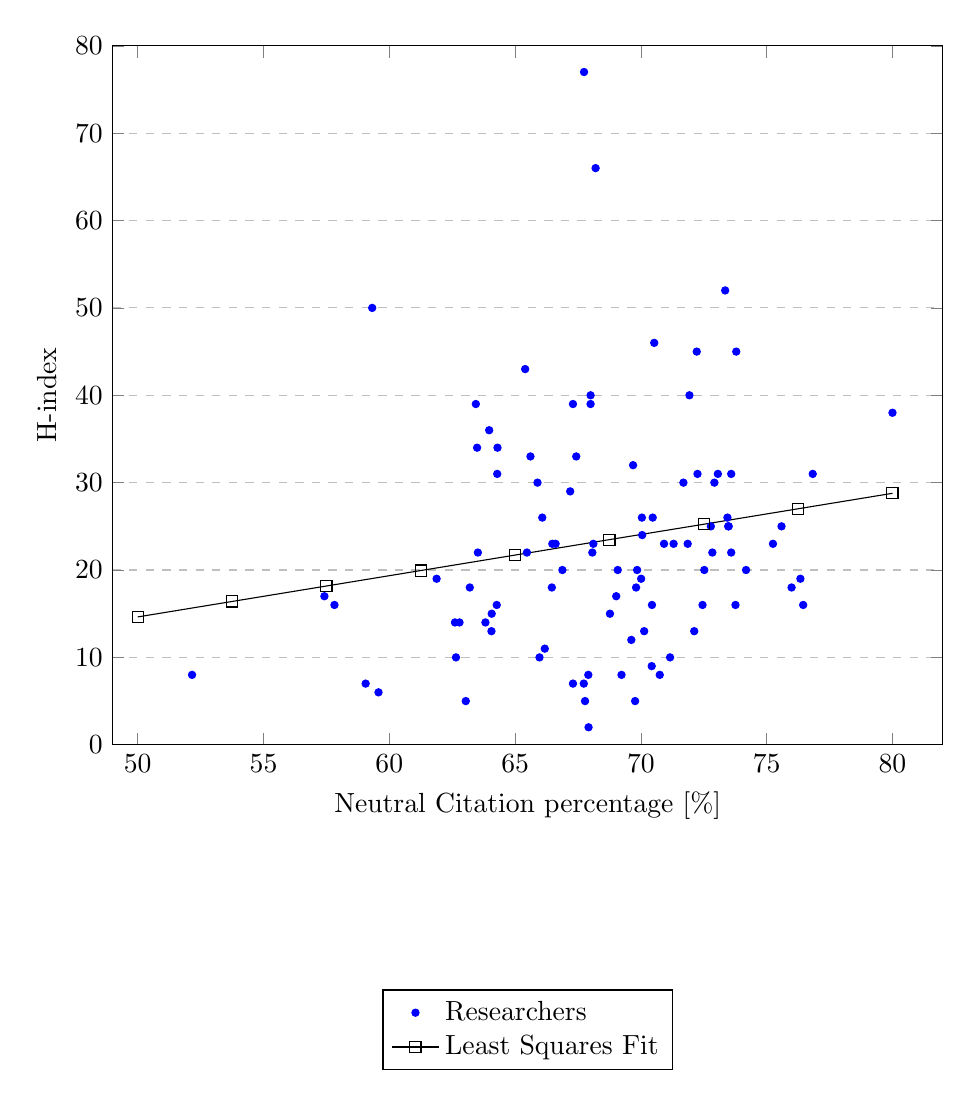
\begin{tikzpicture}
      \begin{axis}[
          width=(1\textwidth),
          xlabel={Neutral Citation percentage [\%]},
          ylabel={H-index},
          xmin=49, xmax=82,
          ymin=0, ymax=80,
          xtick={50, 55, 60, 65, 70, 75, 80},
          ytick={0,10,20,30,40,50,60,70,80},
          ymajorgrids=true,
          grid style=dashed,
      ]
      
      \addplot[
        only marks, color=blue, mark size=1.3pt
        ]
        coordinates {
          (70.44,16)(72.45,16)(67.78,5)(68.11,23)(71.3,23)(72.84,22)(59.06,7)(63.2,18)(73.47,25)(66.18,11)(69.69,32)(73.44,26)(69.81,18)(68.2,66)(68.0,40)(69.77,5)(66.48,23)(62.79,14)(64.06,13)(70.05,24)(70.53,46)(63.44,39)(64.29,31)(67.3,39)(69.02,17)(76.45,16)(69.85,20)(69.62,12)(71.86,23)(71.93,40)(59.32,50)(61.88,19)(57.42,17)(63.52,22)(65.97,10)(70.43,9)(64.07,15)(67.43,33)(65.4,43)(67.73,7)(73.79,45)(70.47,26)(70.92,23)(76.83,31)(64.27,16)(63.97,36)(72.25,31)(66.61,23)(65.47,22)(57.82,16)(72.92,30)(68.0,39)(70.04,26)(63.82,14)(67.74,77)(67.91,8)(69.23,8)(73.59,22)(67.3,7)(72.12,13)(72.78,25)(62.61,14)(64.3,34)(63.49,34)(70.75,8)(75.25,23)(68.77,15)(69.08,20)(73.35,52)(72.22,45)(72.52,20)(66.46,18)(73.06,31)(75.99,18)(73.59,31)(80.0,38)(71.16,10)(63.04,5)(75.59,25)(68.07,22)(62.65,10)(71.69,30)(73.76,16)(65.61,33)(65.89,30)(70.13,13)(73.49,25)(74.18,20)(66.88,20)(67.92,2)(67.19,29)(52.16,8)(66.08,26)(59.57,6)(70.01,19)(76.34,19)
        };
        \addlegendentry{Researchers}
      
      \addplot[
        mark=square,
        ]
        coordinates {
          (50.0,14.63)(53.75,16.4)(57.5,18.17)(61.25,19.94)(65.0,21.71)(68.75,23.48)(72.5,25.24)(76.25,27.01)(80.0,28.78)
        };
        \addlegendentry{Least Squares Fit}
          
      \end{axis}
      \end{tikzpicture}
      \caption{Neutral citation percentage vs. H-index}
      \label{graph:neutral-karma}
    \end{subfigure}
    \caption{Citation purpose percentages vs. H-index of researchers}
    \label{fig:researcher-karma}
\end{figure*}

\begin{figure}
  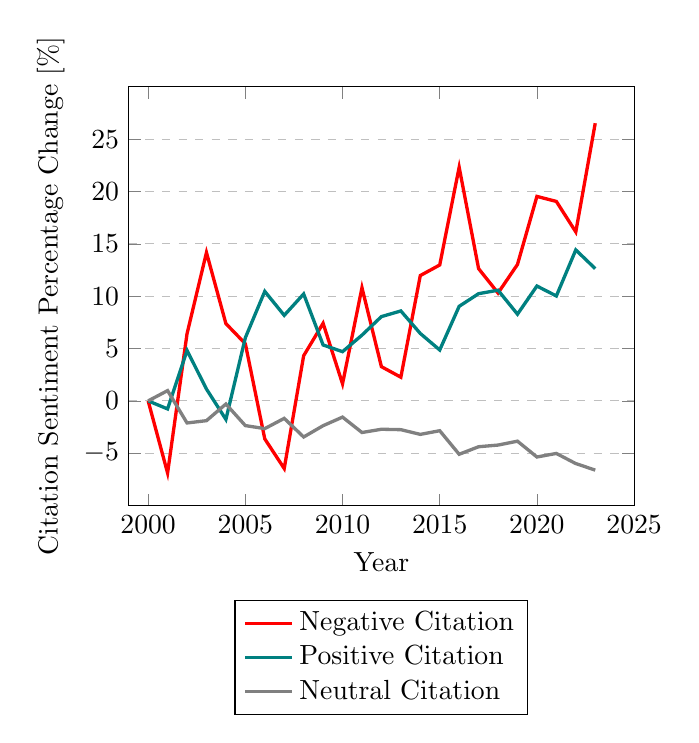
\begin{tikzpicture}
    \begin{axis}[
        /pgf/number format/1000 sep={},
        ylabel={Citation Sentiment Percentage Change [\%]},
        xlabel={Year},
        ymin=-10, ymax=30,
        xmin=1999, xmax=2025,
        ytick={-5, 0, 5, 10, 15, 20, 25}, % 40, 50, 60, 70, 80},
        xtick={2000, 2005, 2010, 2015, 2020, 2025},
        ymajorgrids=true,
        grid style=dashed,
        legend style={at={(0.5,-0.5)},anchor=south},
        every axis plot/.append style={very thick}
    ]
    \addplot[
      red
      ]
      coordinates {
        (2000,0.0)(2001,-6.89)(2002,6.41)(2003,14.17)(2004,7.38)(2005,5.46)(2006,-3.63)(2007,-6.46)(2008,4.31)(2009,7.41)(2010,1.63)(2011,10.81)(2012,3.27)(2013,2.26)(2014,11.97)(2015,12.98)(2016,22.32)(2017,12.63)(2018,10.3)(2019,13.03)(2020,19.53)(2021,19.05)(2022,16.14)(2023,26.52)
      };
      \addlegendentry{Negative Citation}
    
    \addplot[teal]
      coordinates {
        (2000,0.0)(2001,-0.77)(2002,4.82)(2003,1.13)(2004,-1.77)(2005,6.03)(2006,10.46)(2007,8.17)(2008,10.21)(2009,5.34)(2010,4.7)(2011,6.28)(2012,8.05)(2013,8.59)(2014,6.44)(2015,4.86)(2016,9.03)(2017,10.24)(2018,10.57)(2019,8.28)(2020,10.97)(2021,10.02)(2022,14.42)(2023,12.63)
      };
      \addlegendentry{Positive Citation}
    
    \addplot[gray]
      coordinates {
        (2000,0.0)(2001,0.98)(2002,-2.11)(2003,-1.89)(2004,-0.3)(2005,-2.36)(2006,-2.65)(2007,-1.67)(2008,-3.45)(2009,-2.37)(2010,-1.55)(2011,-3.02)(2012,-2.71)(2013,-2.75)(2014,-3.2)(2015,-2.85)(2016,-5.1)(2017,-4.38)(2018,-4.22)(2019,-3.85)(2020,-5.36)(2021,-5.02)(2022,-5.99)(2023,-6.61)
      };
      \addlegendentry{Neutral Citation}
        
    \end{axis}
    \end{tikzpicture}
    \caption{Citation sentiment percentage change throughout years}
    \label{graph:year-karma}
\end{figure}

\begin{figure*}
  \centering
  \begin{subfigure}{0.3\textwidth}
    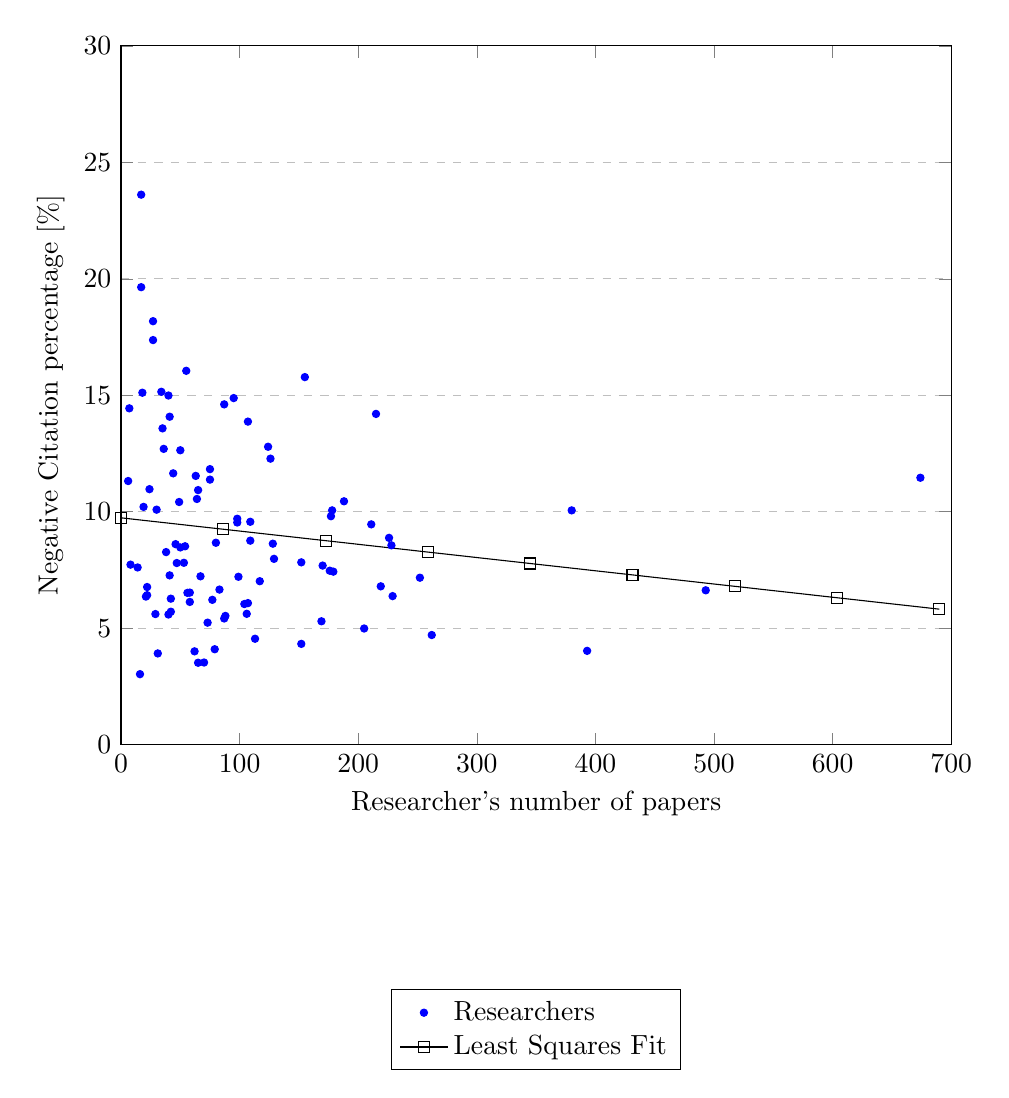
\begin{tikzpicture}
      \begin{axis}[
          width=(1\textwidth),
          ylabel={Negative Citation percentage [\%]},
          xlabel={Researcher's number of papers},
          ymin=0, ymax=30,
          xmin=0, xmax=700,
          ytick={0, 5, 10, 15, 20, 25, 30},
          xtick={0, 100, 200, 300, 400, 500, 600, 700},
          ymajorgrids=true,
          grid style=dashed,
        ]
      
        \addplot[
          only marks, color=blue, mark size=1.3pt
          ]
          coordinates {
            (34,15.15)(64,10.55)(7,14.44)(99,7.21)(109,9.57)(152,7.83)(27,18.18)(54,8.52)(83,6.66)(31,3.92)(211,9.46)(219,6.8)(62,4.01)(674,11.46)(129,7.98)(8,7.73)(75,11.38)(36,12.7)(55,16.05)(58,6.53)(252,7.17)(88,5.53)(226,8.88)(178,10.06)(75,11.83)(87,5.42)(38,8.27)(40,5.59)(113,4.55)(188,10.45)(155,15.78)(41,14.08)(50,12.64)(67,7.23)(30,10.09)(21,6.36)(40,14.99)(95,14.88)(179,7.43)(22,6.77)(176,7.47)(50,8.47)(106,5.62)(262,4.71)(87,14.61)(215,14.2)(169,5.3)(177,9.81)(79,4.1)(47,7.8)(117,7.02)(128,8.63)(98,9.7)(44,11.65)(493,6.63)(35,13.58)(22,6.42)(65,3.52)(19,10.21)(41,7.27)(170,7.69)(27,17.37)(107,13.87)(126,12.28)(24,10.97)(73,5.24)(29,5.61)(77,6.22)(380,10.06)(229,6.38)(58,6.13)(63,11.54)(107,6.08)(56,6.52)(152,4.33)(393,4.03)(16,3.03)(14,7.61)(70,3.53)(49,10.42)(18,15.11)(228,8.56)(46,8.61)(80,8.67)(124,12.79)(53,7.81)(205,4.99)(104,6.04)(65,10.93)(6,11.32)(109,8.76)(17,23.61)(98,9.54)(17,19.64)(42,6.27)(42,5.71)
          };
          \addlegendentry{Researchers}
        
        \addplot[
          mark=square,
          ]
          coordinates {
            (0.0,9.74)(86.25,9.25)(172.5,8.76)(258.75,8.27)(345.0,7.78)(431.25,7.29)(517.5,6.8)(603.75,6.31)(690.0,5.82)
          };
          \addlegendentry{Least Squares Fit}
          
      \end{axis}
    \end{tikzpicture}
    \caption{Negative citation percentage vs. H-index}
    \label{graph:negative-career}
\end{subfigure}
\hfill
\begin{subfigure}{0.3\textwidth}
  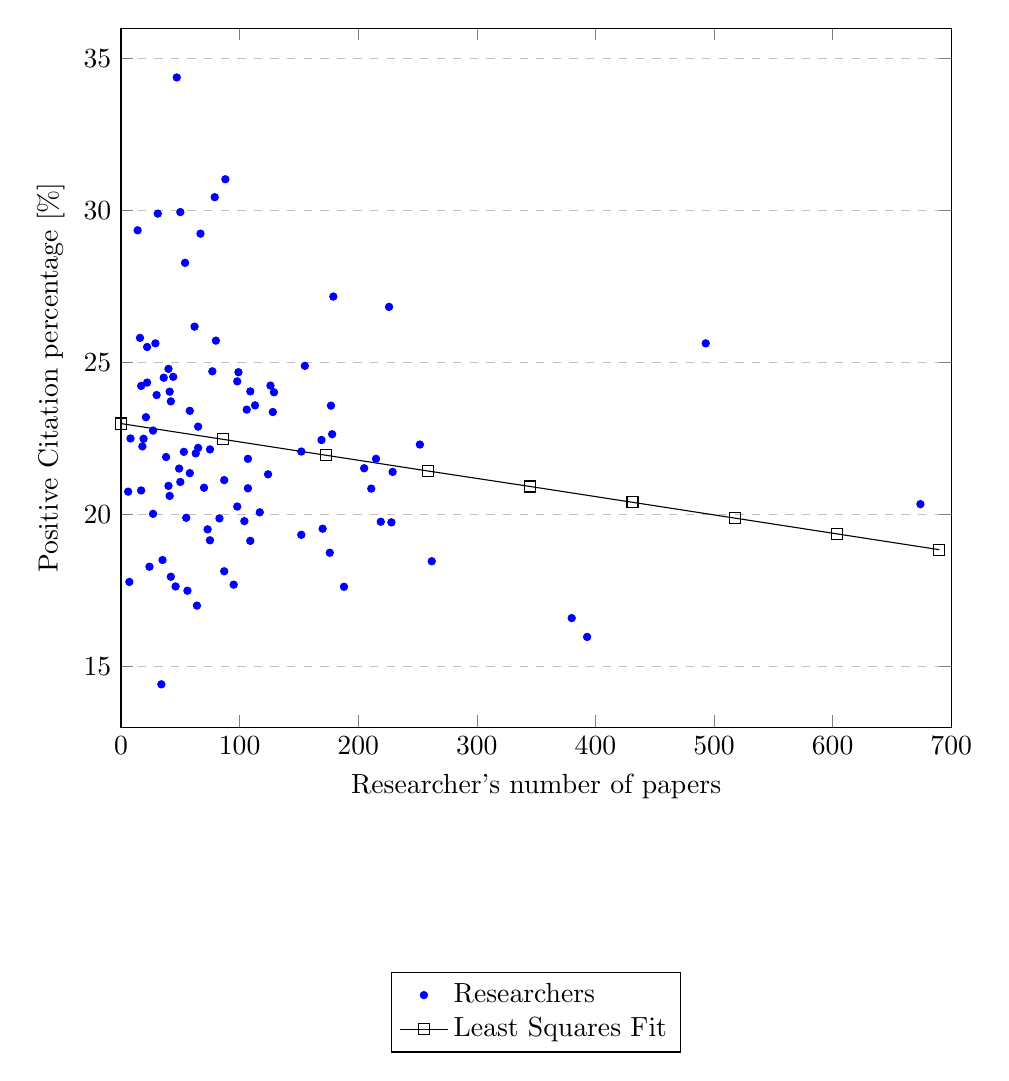
\begin{tikzpicture}
    \begin{axis}[
        width=(1\textwidth),
        ylabel={Positive Citation percentage [\%]},
        xlabel={Researcher's number of papers},
        ymin=13, ymax=36,
        xmin=0, xmax=700,
        ytick={15, 20, 25, 30, 35},
        xtick={0, 100, 200, 300, 400, 500, 600, 700},
        ymajorgrids=true,
        grid style=dashed,
    ]
    
    \addplot[
      only marks, color=blue, mark size=1.3pt
      ]
      coordinates {
        (34,14.41)(64,17.0)(7,17.78)(99,24.68)(109,19.13)(152,19.33)(27,22.76)(54,28.28)(83,19.87)(31,29.9)(211,20.85)(219,19.76)(62,26.18)(674,20.34)(129,24.02)(8,22.5)(75,22.14)(36,24.5)(55,19.89)(58,23.41)(252,22.3)(88,31.03)(226,26.83)(178,22.64)(75,19.15)(87,18.13)(38,21.89)(40,24.79)(113,23.59)(188,17.62)(155,24.89)(41,24.04)(50,29.95)(67,29.24)(30,23.93)(21,23.2)(40,20.94)(95,17.69)(179,27.17)(22,25.51)(176,18.74)(50,21.07)(106,23.45)(262,18.46)(87,21.13)(215,21.83)(169,22.45)(177,23.58)(79,30.44)(47,34.38)(117,20.07)(128,23.37)(98,20.26)(44,24.53)(493,25.63)(35,18.5)(22,24.34)(65,22.89)(19,22.49)(41,20.61)(170,19.53)(27,20.02)(107,21.83)(126,24.24)(24,18.28)(73,19.51)(29,25.63)(77,24.71)(380,16.59)(229,21.4)(58,21.36)(63,22.01)(107,20.86)(56,17.49)(152,22.07)(393,15.97)(16,25.81)(14,29.35)(70,20.88)(49,21.51)(18,22.24)(228,19.74)(46,17.63)(80,25.72)(124,21.32)(53,22.06)(205,21.52)(104,19.78)(65,22.19)(6,20.75)(109,24.05)(17,24.23)(98,24.38)(17,20.79)(42,23.72)(42,17.95)
      };
      \addlegendentry{Researchers}
    
    \addplot[
      mark=square,
      ]
      coordinates {
        (0.0,22.99)(86.25,22.47)(172.5,21.95)(258.75,21.43)(345.0,20.92)(431.25,20.4)(517.5,19.88)(603.75,19.36)(690.0,18.84)
      };
      \addlegendentry{Least Squares Fit}
        
    \end{axis}
    \end{tikzpicture}
    \caption{Positive citation percentage vs. H-index}
    \label{graph:positive-career}
  \end{subfigure}
  \hfill
  \begin{subfigure}{0.3\textwidth}
    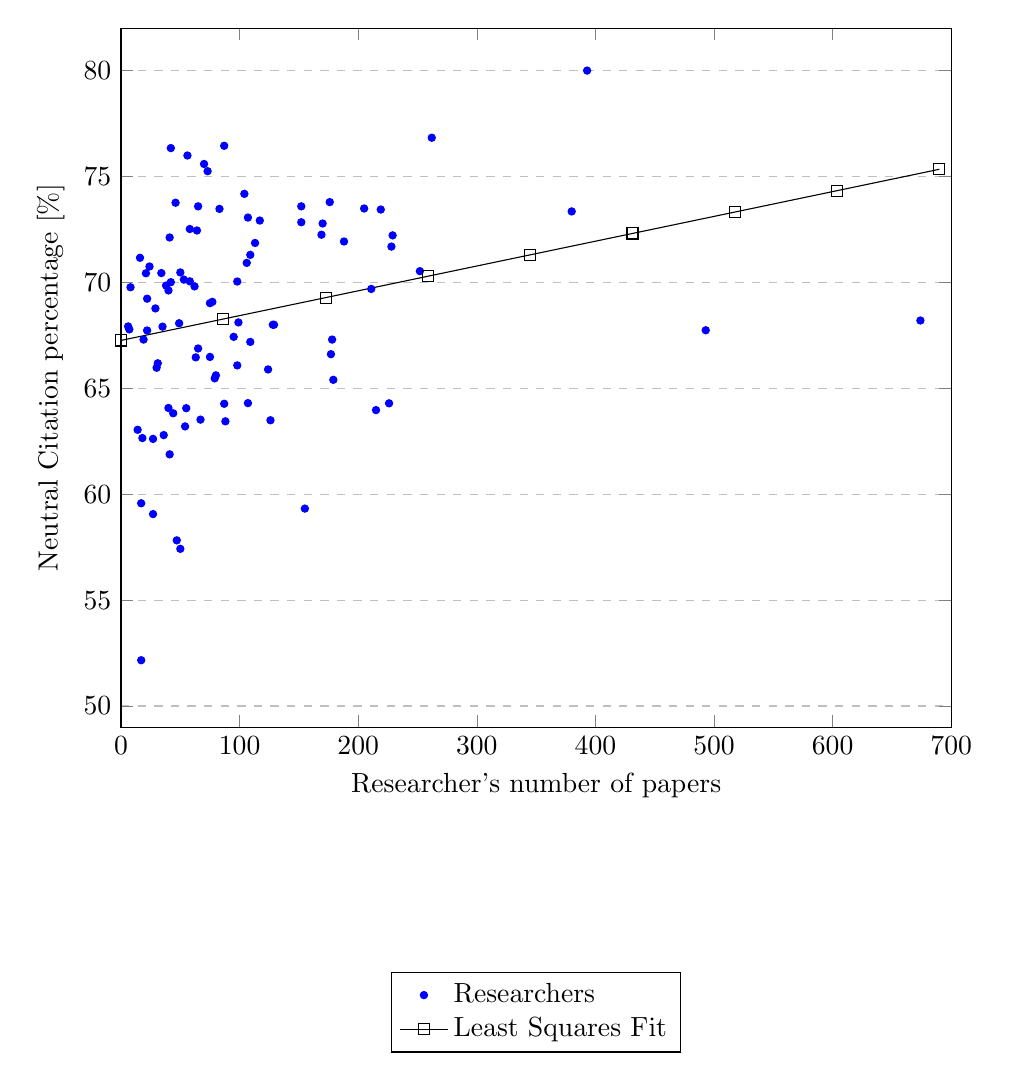
\begin{tikzpicture}
      \begin{axis}[
          width=(1\textwidth),
          ylabel={Neutral Citation percentage [\%]},
          xlabel={Researcher's number of papers},
          ymin=49, ymax=82,
          xmin=0, xmax=700,
          ytick={50, 55, 60, 65, 70, 75, 80},
          xtick={0, 100, 200, 300, 400, 500, 600, 700},
          ymajorgrids=true,
          grid style=dashed,
      ]
      
      \addplot[
        only marks, color=blue, mark size=1.3pt
        ]
        coordinates {
          (34,70.44)(64,72.45)(7,67.78)(99,68.11)(109,71.3)(152,72.84)(27,59.06)(54,63.2)(83,73.47)(31,66.18)(211,69.69)(219,73.44)(62,69.81)(674,68.2)(129,68.0)(8,69.77)(75,66.48)(36,62.79)(55,64.06)(58,70.05)(252,70.53)(88,63.44)(226,64.29)(178,67.3)(75,69.02)(87,76.45)(38,69.85)(40,69.62)(113,71.86)(188,71.93)(155,59.32)(41,61.88)(50,57.42)(67,63.52)(30,65.97)(21,70.43)(40,64.07)(95,67.43)(179,65.4)(22,67.73)(176,73.79)(50,70.47)(106,70.92)(262,76.83)(87,64.27)(215,63.97)(169,72.25)(177,66.61)(79,65.47)(47,57.82)(117,72.92)(128,68.0)(98,70.04)(44,63.82)(493,67.74)(35,67.91)(22,69.23)(65,73.59)(19,67.3)(41,72.12)(170,72.78)(27,62.61)(107,64.3)(126,63.49)(24,70.75)(73,75.25)(29,68.77)(77,69.08)(380,73.35)(229,72.22)(58,72.52)(63,66.46)(107,73.06)(56,75.99)(152,73.59)(393,80.0)(16,71.16)(14,63.04)(70,75.59)(49,68.07)(18,62.65)(228,71.69)(46,73.76)(80,65.61)(124,65.89)(53,70.13)(205,73.49)(104,74.18)(65,66.88)(6,67.92)(109,67.19)(17,52.16)(98,66.08)(17,59.57)(42,70.01)(42,76.34)
        };
        \addlegendentry{Researchers}
      
      \addplot[
        mark=square,
        ]
        coordinates {
          (0.0,67.26)(86.25,68.27)(172.5,69.28)(258.75,70.29)(345.0,71.3)(431.25,72.31)(517.5,73.32)(603.75,74.33)(690.0,75.34)
        };
        \addlegendentry{Least Squares Fit}
          
      \end{axis}
      \end{tikzpicture}
      \caption{Neutral citation percentage vs. H-index}
      \label{graph:neutral-career}
    \end{subfigure}
    \caption{Citation purpose percentages vs. researchers' number of papers}
    \label{fig:researcher-career}
\end{figure*}

\begin{figure}
  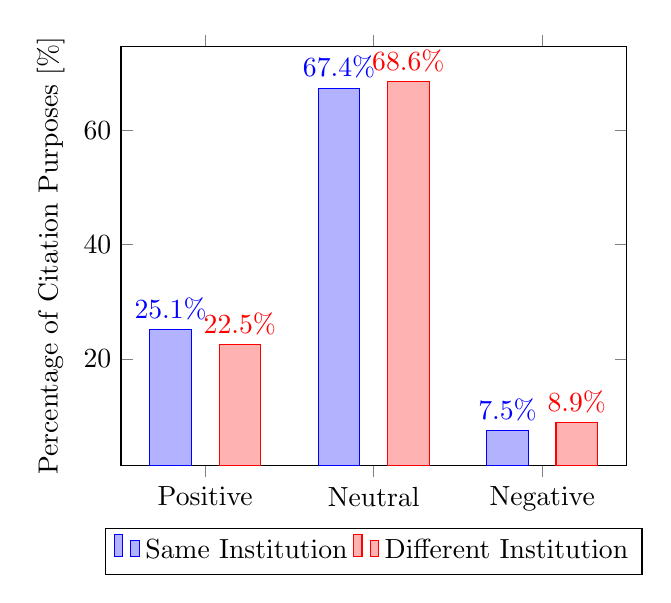
\begin{tikzpicture}
    \begin{axis}[
        ybar=10pt,
        bar width=15pt,
        enlarge x limits=0.25,
        legend style={at={(0.5,-0.15)},
          anchor=north,legend columns=-1},
        ylabel={Percentage of Citation Purposes [\%]},
        symbolic x coords={Positive,Neutral,Negative},
        xtick=data,
        nodes near coords={\pgfmathprintnumber\pgfplotspointmeta\%},
        nodes near coords align={vertical},
        ]
    \addplot coordinates {(Positive,25.1) (Neutral,67.4) (Negative,7.5)};
    \addplot coordinates {(Positive,22.5) (Neutral,68.6) (Negative,8.9)};
    \legend{Same Institution,Different Institution}
    \end{axis}
    \end{tikzpicture}
    \caption{Citation purpose percentages within and outside of the institution}
    \label{graph:institute-karma}
\end{figure}

We see a distribution of 21.59\% positive, 65.58\% neutral, 8.47\% negative, and 4.37\% bad context in Figure \ref{graph:distribution}. This data might not represent the actual distribution of citation sentiments in computer science because all the papers being cited belongs to University of Waterloo professors. Given that University of Waterloo has a relatively high ranking in computer science it is possible that the distribution of citation sentiments is skewed towards positive and neutral.

\subsection{RQ1: Does Citation Karma Exists?}
When we graph the citation sentiment percentages against the H-index of researchers, we see a negative correlation between negative citation percentage and H-index in Figure \ref{graph:negative-karma}. We also see a very slight negative correlation between positive citation percentage and H-index in Figure \ref{graph:positive-karma}. However, we see a positive correlation between neutral citation percentage and H-index in Figure \ref{graph:neutral-karma}. While it looks easy to jump into the conclusion that there is a karma effect meaning, when you give too much negative references you will get lower number of citations. However, this could be related to the career stage of the researcher as we will see in the next section.

\subsection{RQ2: How does the citation sentiment percentages change throughout the career of a researcher?}
We decided to use the number of papers published by a researcher as an indication of the career stage of the researcher. When we graph the researchers citation sentiment percentages and their number of published papers we get the graphs in Figure \ref{fig:researcher-career}, we can see that as the researchers publish more papers the negative and positive citation percentages decrease and neutral citation percentages increase. We can hypothesize that as the researchers get more experienced they tend to give more neutral references. This can also explain the negative correlation between the negative and positive citation percentage and H-index and positive correlation between neutral citation percentage and H-index. This is because H-index is also an indirect measure of the career stage of a researcher, as more experienced researchers tend to have higher H-indexes.

\subsection{RQ3: How did the distribution of citation sentiments changed over time?}
We calculated the average citation sentiment percentages for each year from 2000 to 2023, these citations include both the citations the Waterloo professors received and the citations they gave. We then graphed the percentage changes of the three classes in Figure \ref{graph:year-karma}. As you can see there is a consistent increase in positive and negative citation percentages and a consistent decrease in neutral citation percentage. This could potentially mean that the computer science community is getting more polarized over time.

\subsection{RQ4: Does being in the same institution affect the citation sentiment distribution?} 
We calculated the average citation sentiment percentages for citations given to University of Waterloo professors by other University of Waterloo professors and by professors from other institutions. We then graphed the results in Figure \ref{graph:institute-karma}. We can see that the distribution of citation sentiments is very similar for both cases. However, we can see a 2.6\% increase in positive citation percentage and a 1.4\% decrease in negative citation percentage when the citation is given by a professor from the same institution. This could potentially point to a slight positive bias towards professors from the same institution.

\section{Conclusion}
In conclusion, our analysis of citation sentiments among University of Waterloo professors in computer science reveals intriguing patterns. While the overall distribution suggests a predominantly positive and neutral sentiment, it's essential to acknowledge the potential skew introduced by the university's high ranking. Examining the existence of "Citation Karma," we observed a nuanced relationship between citation sentiments and researchers' H-index, hinting at a possible correlation with career stage.

Exploring the evolution of sentiments throughout researchers' careers, we found a tendency for more experienced researchers to provide increasingly neutral references, aligning with the observed correlations. The temporal analysis indicates a growing polarization in the computer science community, reflected in rising positive and negative citation percentages alongside a decline in neutral citations over time.

Furthermore, our investigation into the influence of institutional affiliation on citation sentiment distribution suggests a subtle positive bias when citations originate from the same institution. These findings contribute to a deeper understanding of the dynamics shaping scholarly communication within a specific academic community.

In summary, our study sheds light on the complex interplay of factors influencing citation sentiments, ranging from individual career stages to institutional affiliations and temporal shifts. These insights encourage further exploration into the evolving landscape of scholarly interactions and their implications for the dynamics of academic discourse.

%%
%% The acknowledgments section is defined using the "acks" environment
%% (and NOT an unnumbered section). This ensures the proper
%% identification of the section in the article metadata, and the
%% consistent spelling of the heading.
% \begin{acks}
% To Robert, for the bagels and explaining CMYK and color spaces.
% \end{acks}

%%
%% The next two lines define the bibliography style to be used, and
%% the bibliography file.
\bibliographystyle{ACM-Reference-Format}
\bibliography{sample-base}


%%
%% If your work has an appendix, this is the place to put it.
\appendix

\section{Classification Prompt Template}
\label{appendix:classification-prompt}
The following is a set of citation sentiment categories, each category name is followed by a description of the category and some examples of in-text citation contexts that belongs to this category.

\begin{itemize}
  \item \textbf{Name}: Positive
  
  \textbf{Description}: A citing sentence is classified as "positive" when it mentions the strength of the cited approach, positively criticizes the cited approach, positively evaluates the cited source, uses the cited source as a starting point or motivation and extends on the cited work, or when the results, claims of the citing work substantiate, verify the cited paper and support each other.
  
  \textbf{Example 1}: Researchers [13] have presented a Secure and Efficient Topology Discovery Protocol (sOFTDP) that shifts a part of the link discovery to the SDN switch.
  
  \textbf{Example 2}: To obtain more precise and descriptive topics, we further conducted GuidedLDA [24] using some of the most salient keywords selected from our initial LDA results.
  
  \item \textbf{Name}: Negative
  
  \textbf{Description}: A citing sentence is classified as "negative" when it mentions the weakness of the cited approach, negatively criticizes the cited approach, negatively evaluates the cited source.
  
  \textbf{Example 1}: Most of the existing literature on the execution cost problem focus on markets where only one investor trades (for instance see [3, 4, 5, 6, 8, 9]).
  
  \textbf{Example 2}: With nonlinear CI test, LPCMCI is computationally too expensive to be compared when the number of nodes is large.

  \item \textbf{Name}: Neutral
  
  \textbf{Description}: A citing sentence is classified as "neutral" when it is a neutral description of the cited work. Use this category when there is no strong criticism negatively or positively.
  
  \textbf{Example 1}: Since the inception of spam, many companies and research teams have combined their efforts to fight against spam deliveries using different approaches and methods [1].
  
  \textbf{Example 2}: Conventional approaches adopt fine-tuned generative models (Zhong et al., 2020b; Guo et al., 2021; Wang et al., 2021a, inter alia ) as input generators, with a semantic parser (e.g., PCFG grammar) for sampling symbolic outputs.
  
  \item \textbf{Name}: Bad Context
  
  \textbf{Description}: A citing sentence is classified as "bad context" when the given context is not enough to classify the citation or it does not include any citation.
  
  \textbf{Example 1}: But then, the sum of welfare lost + retained is the optimum welfare and is bounded.
  
  \textbf{Example 2}: Furthermore, since step (4) did not return FAIL, we must have g; a divisor of all entries in V' and W' hence JV contains only polynomial entries.  
\end{itemize}

Classify the following in text citation into one of these categories. First, type 'THINKING:' and write your reasoining step by step. Then type 'ANSWER:' and give your answer in a single word.

\{Citation Context\}


\end{document}
\endinput
%%
%% End of file `sample-sigconf.tex'.
